\documentclass{article}

\usepackage[submission]{colm2026_conference}
\usepackage{microtype}
\usepackage{graphicx}
\usepackage{booktabs}
\usepackage{amsmath}
\usepackage{amssymb}
\usepackage{xcolor}
\usepackage{multirow}
\usepackage{lineno}

\usepackage{hyperref}
\definecolor{darkblue}{rgb}{0, 0, 0.5}
\hypersetup{colorlinks=true, citecolor=darkblue, linkcolor=darkblue, urlcolor=darkblue}

\usepackage{mathtools}
\usepackage{amsthm}

\title{Representational Commitment: \\ When Hidden States Predict Behavioral Consistency in LLM Agents}

\author{Anonymous Author(s)}

\begin{document}

\ifcolmsubmission
\linenumbers
\fi

\maketitle

\begin{abstract}
LLM-based agents exhibit behavioral inconsistency: the same agent given the same task produces different reasoning trajectories across runs. We investigate whether this inconsistency has a signature in internal representations. Using Llama-3.1-70B on a ReAct question-answering task (100 questions, 10 runs each, 1{,}000 total trajectories), we find that \emph{activation similarity}---pairwise cosine similarity of hidden states across runs at a given step---predicts behavioral consistency ($r = -0.35$, 95\% CI $[-0.48, -0.17]$, permutation $p < 0.001$). Higher similarity indicates the model has not updated its representations in response to observations, remaining in an undifferentiated state from which future behavior diverges. We call this \textbf{representational commitment}: the degree to which a model integrates observations into its internal state. The signal emerges at step~4 of the agent trajectory, spans layers 32--80, and \emph{strengthens} after controlling for task difficulty (partial $r = -0.45$, 95\% CI $[-0.59, -0.29]$, $p < 10^{-5}$). Questions in the lowest activation-similarity quartile show 4.1$\times$ higher behavioral variance than those in the highest quartile (Cohen's $d = 1.01$, $p = 0.002$). It is not explained by question length, context size, or other simple baselines. Notably, the signal predicts \emph{between-run consistency} but not \emph{per-run correctness} (probing AUC $\approx 0.5$), establishing it as a fundamentally relational property of agent representations. We validate cross-model on Qwen~2.5~72B ($r = -0.65$, 95\% CI $[-0.74, -0.55]$) and Phi-3-Medium-14B ($r = -0.36$, 95\% CI $[-0.52, -0.17]$), a structurally different model (14B parameters, 40 layers, $d{=}5120$), confirming the finding generalizes across architectures and scales. Cross-benchmark validation on StrategyQA ($r = -0.83$, 95\% CI $[-0.90, -0.76]$, $n{=}50$) confirms generalization to a different task type, with the commitment juncture shifting to step~3 consistent with shorter reasoning chains. A runtime monitor using step-4 hidden states achieves AUROC up to 0.97 for predicting consistency. A prompting intervention that induces explicit commitment at step~3 reduces behavioral CV by 16\% ($p = .037$, $d = 0.21$) without affecting accuracy, with the effect concentrating on originally-inconsistent questions (CV reduction of 30\%, $p < .001$). To our knowledge, this is the first work connecting agent behavioral reliability to hidden-state geometry and demonstrating that inducing representational commitment improves agent consistency.
\end{abstract}

%%%%%%%%%%%%%%%%%%%%%%%%%%%%%%%%%%%%%%%%%%%%%%%%%%%%%%%%%%%%%%%%%%%%%%%%%%%%%%%
\section{Introduction}
%%%%%%%%%%%%%%%%%%%%%%%%%%%%%%%%%%%%%%%%%%%%%%%%%%%%%%%%%%%%%%%%%%%%%%%%%%%%%%%

LLM-based agents---systems combining language models with tool use and multi-step reasoning \citep{react, cot}---face a critical reliability concern: \emph{behavioral inconsistency}. When given the same task multiple times with non-zero sampling temperature, agents produce different action sequences, explore different reasoning paths, and often reach different conclusions. This is not merely a theoretical concern: production agent systems are typically evaluated on single runs, yet the same system can produce correct answers on one run and incorrect answers on another for the same input. Inconsistency complicates deployment, debugging, and benchmarking.

Recent work has begun to characterize this phenomenon. Multi-run evaluation reveals that the majority of agent divergence occurs at early decision points such as the first search query \citep{anonymous2026a}, and that behavioral consistency amplifies outcomes---both positive and negative---rather than guaranteeing correctness \citep{anonymous2026b}. But these studies measure what agents \emph{do} without examining what happens \emph{inside} the model. A deeper question remains: does behavioral consistency have a measurable signature in the model's internal representations?

We answer affirmatively. Extracting hidden states from Llama-3.1-70B \citep{llama3} during ReAct \citep{react} question-answering on HotpotQA \citep{hotpotqa}, we find that cross-run \emph{activation similarity}---how similar hidden states are across multiple runs of the same question---predicts downstream behavioral consistency. We introduce the concept of \textbf{representational commitment}: when a model integrates observations into differentiated internal states, each run follows a focused strategy and behavior is consistent; when internal states remain undifferentiated despite receiving different observations, the model has not committed, and behavior diverges.

Our contributions:
\begin{enumerate}
    \item Activation similarity at step~4 predicts consistency ($r = -0.35$, 95\% CI $[-0.48, -0.17]$, permutation $p < 0.001$, $n{=}100$), \emph{strengthening} after difficulty controls (partial $r = -0.45$, 95\% CI $[-0.59, -0.29]$, $p < 10^{-5}$). Quartile analysis reveals a 4.1$\times$ effect: questions with lowest similarity show mean CV $= 0.25$ vs.\ $0.06$ for highest ($d = 1.01$).
    \item The signal has temporal and spatial specificity: absent at steps 1--2, peaking at step~4, spanning layers 32--80.
    \item The signal predicts \emph{between-run consistency} but not \emph{per-run correctness} (probing AUC~$\approx 0.5$), distinguishing committed from uncommitted states but not correct from incorrect ones.
    \item Cross-model validation on Qwen~2.5~72B ($r = -0.65$, 95\% CI $[-0.74, -0.55]$) and Phi-3-Medium-14B ($r = -0.36$, 95\% CI $[-0.52, -0.17]$ at step~4; $r = -0.58$, 95\% CI $[-0.72, -0.41]$ at step~5), a structurally different 14B model with 40 layers and $d{=}5120$, confirms the signal generalizes across model families and scales.
    \item Cross-benchmark validation on StrategyQA ($r = -0.83$ at step~3, 95\% CI $[-0.90, -0.76]$, $n{=}50$) confirms the signal generalizes to implicit-reasoning yes/no tasks, with the commitment juncture shifting earlier consistent with shorter reasoning chains.
    \item A runtime monitor using step-4 hidden states achieves AUROC up to 0.97 (Llama) and 0.93 (Qwen) for predicting behavioral consistency via LOOCV, substantially outperforming surface-level baselines.
    \item A prompting intervention inducing explicit commitment at step~3 reduces behavioral CV by 16\% ($d = 0.21$, $p = .037$) without affecting accuracy, with the effect concentrating on originally-inconsistent questions (30\% CV reduction, $p < .001$).
\end{enumerate}

%%%%%%%%%%%%%%%%%%%%%%%%%%%%%%%%%%%%%%%%%%%%%%%%%%%%%%%%%%%%%%%%%%%%%%%%%%%%%%%
\section{Related Work}
%%%%%%%%%%%%%%%%%%%%%%%%%%%%%%%%%%%%%%%%%%%%%%%%%%%%%%%%%%%%%%%%%%%%%%%%%%%%%%%

\textbf{Behavioral consistency in agents.} \citet{anonymous2026a} introduced multi-run behavioral consistency as an agent reliability metric on HotpotQA, finding a 32--55 percentage point accuracy gap between consistent and inconsistent runs. \citet{anonymous2026b} extended this to SWE-bench, revealing that consistency amplifies outcomes rather than guaranteeing correctness. Self-consistency \citep{wang2023selfconsistency} leverages output-level variance via majority voting but does not examine internal representations.

\textbf{Probing LLM representations.} Hidden states encode truth \citep{burns2023discovering, marks2024geometry}, model confidence \citep{kadavath2022language}, and answer correctness in reasoning models \citep{stickland2024reasoning}. \citet{gnosis} showed that lightweight probes can detect incorrect generations from hidden states in single-turn settings. We extend probing to \emph{multi-step agentic settings} and find it predicts consistency but, notably, not per-run correctness.

\textbf{Representation engineering.} \citet{zou2023repe} introduced representation reading and control; \citet{turner2023steering} demonstrated activation steering for behavioral modification. \citet{anthropic_persona} extracted ``persona vectors'' encoding character traits, and \citet{anthropic_axis} identified an ``assistant axis'' governing default model behavior. Our work identifies a new representational property---commitment---that may constitute another such axis in activation space.

%%%%%%%%%%%%%%%%%%%%%%%%%%%%%%%%%%%%%%%%%%%%%%%%%%%%%%%%%%%%%%%%%%%%%%%%%%%%%%%
\section{Method}
%%%%%%%%%%%%%%%%%%%%%%%%%%%%%%%%%%%%%%%%%%%%%%%%%%%%%%%%%%%%%%%%%%%%%%%%%%%%%%%

\textbf{Agent and task.} We deploy Llama-3.1-70B-Instruct \citep{llama3} in a ReAct \citep{react} agent on HotpotQA \citep{hotpotqa}. The agent iterates Thought $\rightarrow$ Action $\rightarrow$ Observation using Search, Retrieve, and Finish tools. We select 100 questions from the validation set: 50 ``easy'' (comparison questions with yes/no answers) and 50 ``hard'' (multi-hop requiring 2+ retrieval steps). Each question is run 10 times with temperature $T{=}0.5$ and maximum 25 steps, yielding 988 total trajectories.\footnote{12 runs excluded due to incomplete hidden state extraction.} At step~4 (the primary analysis step), 99 of 100 questions have sufficient data; one question's runs all terminated by step~3.

\textbf{Hidden state extraction.} The model runs on 8$\times$80GB GPUs with pipeline parallelism (10 layers per GPU). At every agent step, we extract the hidden state at the last token position from layers $\ell \in \{0, 8, 16, \ldots, 80\}$, producing $\mathbf{h}_{\ell}^{(s)} \in \mathbb{R}^{8192}$ per step $s$ and layer $\ell$.

\textbf{Behavioral consistency.} We measure the coefficient of variation (CV) of step counts across the 10 runs of each question. Lower CV indicates more consistent behavior.

\textbf{Activation similarity.} For each question $q$ at step $s$ and layer $\ell$, we compute the mean pairwise cosine similarity across runs:
\begin{equation}
\text{Sim}_q^{(s,\ell)} = \binom{n}{2}^{-1} \sum_{i < j} \cos\!\left(\mathbf{h}_{\ell,i}^{(s)},\; \mathbf{h}_{\ell,j}^{(s)}\right)
\end{equation}
where $n$ is the number of runs with hidden states at step $s$. We examine the Pearson correlation between $\text{Sim}_q^{(s,\ell)}$ and $\text{CV}_q$ across all questions.

%%%%%%%%%%%%%%%%%%%%%%%%%%%%%%%%%%%%%%%%%%%%%%%%%%%%%%%%%%%%%%%%%%%%%%%%%%%%%%%
\section{Results}
%%%%%%%%%%%%%%%%%%%%%%%%%%%%%%%%%%%%%%%%%%%%%%%%%%%%%%%%%%%%%%%%%%%%%%%%%%%%%%%

\subsection{Activation Similarity Predicts Consistency}

Figure~\ref{fig:heatmap} shows the correlation between activation similarity and behavioral CV across all step--layer combinations. A negative correlation emerges at step~4 across layers 32--80, peaking at layer~40 ($r = -0.348$, 95\% CI $[-0.48, -0.17]$, $p = 0.0006$). A 10{,}000-iteration permutation test confirms significance at all seven sampled layers from 32 to 80 (all permutation $p < 0.002$; full results in Table~\ref{tab:permutation}, Appendix~\ref{app:permutation}).

\begin{figure}[t]
\centering
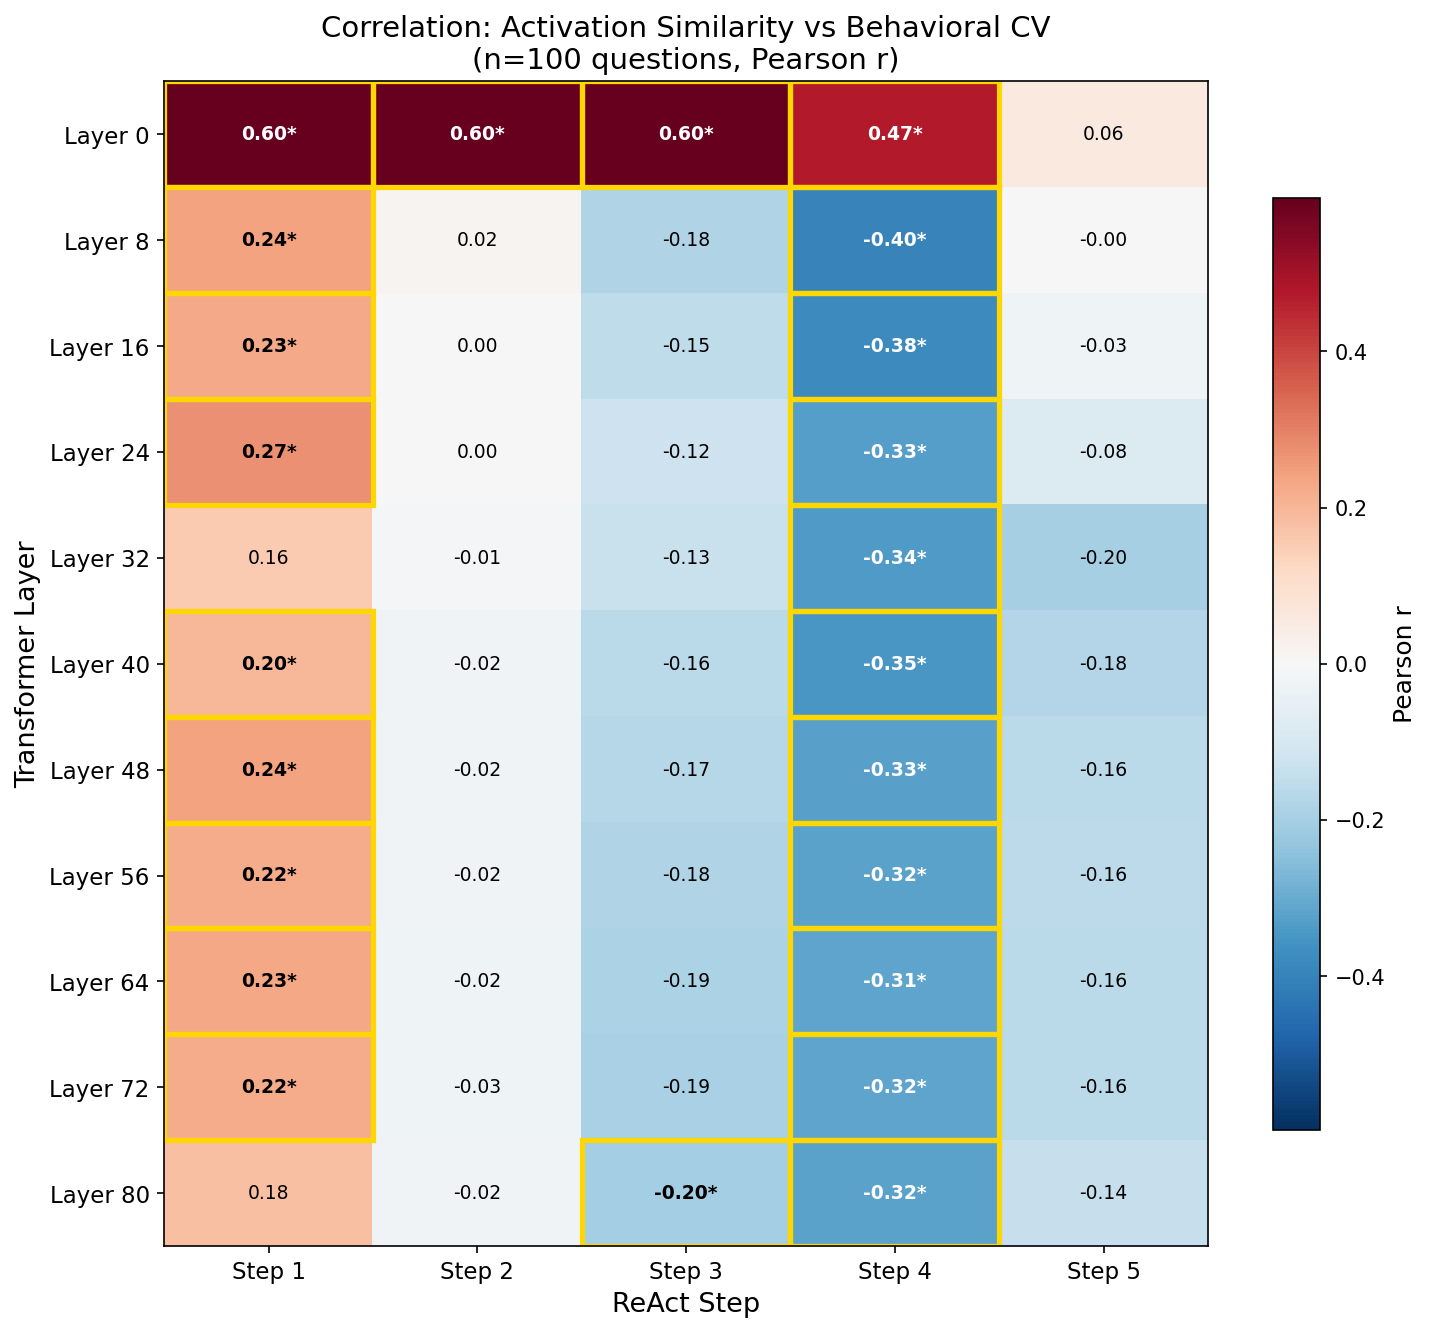
\includegraphics[width=\columnwidth]{figures/step_layer_heatmap_100q.png}
\caption{Pearson $r$ between activation similarity and behavioral CV across steps and layers ($n = 99$; one question excluded at step~4 as all runs terminated before this step). Gold borders indicate $p < 0.05$. The signal concentrates at step~4 across layers 32--80.}
\label{fig:heatmap}
\end{figure}

\textbf{Why does high similarity predict inconsistency?} By step~4, each run has taken 3 actions and received different observations (different search results, different retrieved documents). When hidden states remain similar \emph{despite} these different inputs, the model has not incorporated the observations into its internal state---it remains in a generic, uncommitted representation. Without a committed strategy, sampling perturbations have no anchor, and trajectories scatter. Conversely, when hidden states \emph{differentiate} in response to observations, each run has integrated evidence into a specific interpretation and proceeds consistently.

\subsection{Temporal Profile}

Figure~\ref{fig:step_progression} shows the correlation at layer~40 across steps. The signal is absent at steps 1--2, strengthens at step~3, peaks at step~4 ($r = -0.348$), and weakens at step~5. This trajectory aligns with \citet{anonymous2026a}, who found that 69\% of behavioral divergence begins at step~2. The representational commitment signal appears two steps later, capturing the model's response to the accumulated evidence.

\begin{figure}[t]
\centering
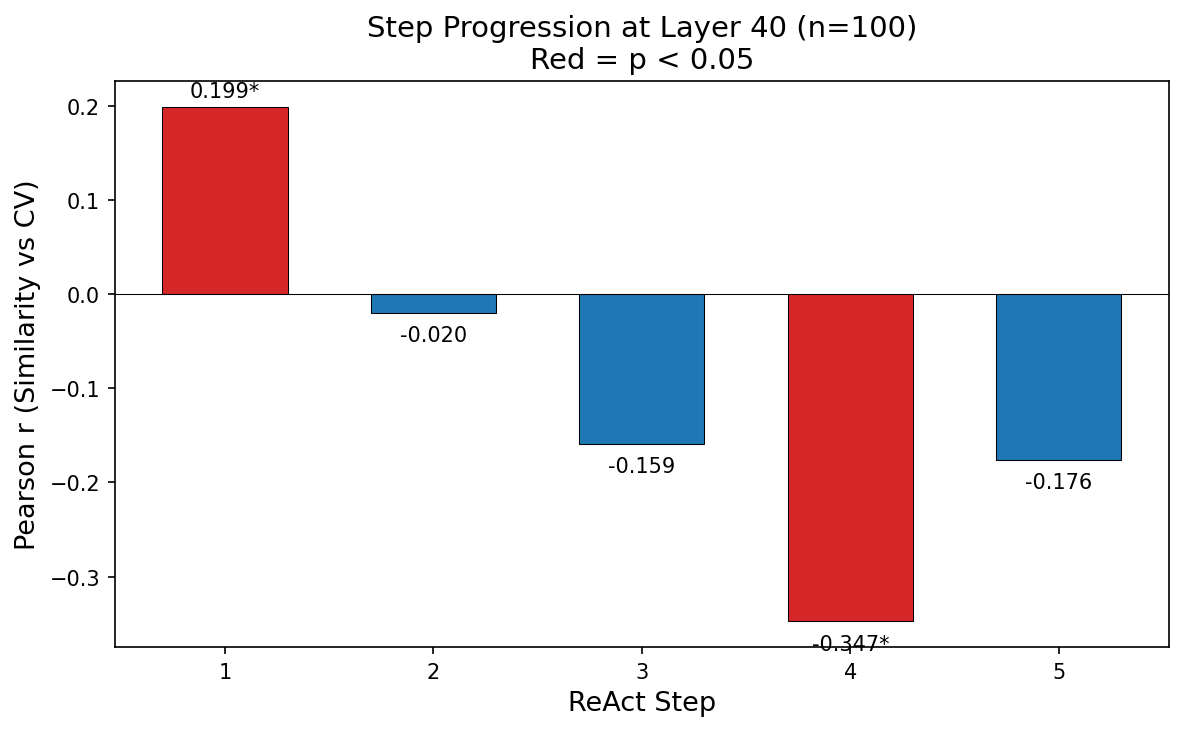
\includegraphics[width=\columnwidth]{figures/step_progression_layer40_100q.png}
\caption{Correlation between activation similarity and CV at layer~40 across steps. The consistency signal peaks at step~4.}
\label{fig:step_progression}
\end{figure}

\subsection{Controlling for Task Difficulty}

Both activation similarity and CV could be driven by task difficulty, creating a spurious correlation. We address this with partial correlation, controlling for question accuracy and a binary difficulty label. The partial correlation \emph{increases} from $r = -0.35$ to $r = -0.45$ (95\% CI $[-0.59, -0.29]$, $p < 10^{-5}$) at layer~40, with all layers 32--80 strengthening after control (partial $r$ range: $-0.38$ to $-0.46$; full table in Appendix~\ref{app:partial}). Task difficulty was partially \emph{suppressing} the signal: once its shared variance with both similarity and CV is removed, the direct relationship becomes clearer. This confirms the signal reflects a genuine representational property independent of task characteristics.

\subsection{Ruling Out Simple Baselines}

We compare hidden state similarity against simpler potential predictors of consistency (full results in Table~\ref{tab:baselines_full}, Appendix~\ref{app:baselines}). No input-level feature---question length ($r = 0.10$, $p = .31$), context size ($r = 0.04$, $p = .66$), or thought length ($r = 0.12$, $p = .24$)---predicts CV. A multiple regression (CV $\sim$ similarity + question length + accuracy) yields $R^2 = 0.30$; similarity ($t = -4.73$, $p < 10^{-5}$) and accuracy ($t = -4.41$, $p < 10^{-4}$) are the only significant predictors.

\subsection{Boundaries of the Signal}

\textbf{Per-run correctness.} Linear probes fail to predict per-run correctness from hidden states (AUC 0.34--0.56 across all configurations including single-turn generation), because correctness is primarily question-determined (64 questions are 10/10 correct, 23 are 0/10). The consistency signal is a \emph{between-run relational} property, not a within-run absolute one.

\textbf{Hard vs.\ easy questions.} The signal is driven by easy questions ($r = -0.57$, $p < 10^{-5}$, $n = 50$) rather than hard ($r = -0.02$, $p = 0.88$, $n = 44$). To explain this, we classify hard questions into commitment categories: \emph{committed-correct} (accuracy $\geq 0.8$), \emph{committed-wrong} (accuracy $\leq 0.2$, CV $\leq 0.15$), and \emph{uncommitted-wrong} (accuracy $\leq 0.2$, CV $> 0.15$). Committed-wrong questions show activation similarity indistinguishable from committed-correct (Llama: $0.935$ vs.\ $0.903$, $p = 0.30$; Qwen: $0.968$ vs.\ $0.952$, $p = 0.46$). Representational commitment is \emph{correctness-agnostic}: the model converges on stable representations whether the answer is right or wrong, collapsing the linear relationship within hard questions (Figure~\ref{fig:commitment_categories}; see also Figure~\ref{fig:tsne} in Appendix~\ref{app:tsne} for a t-SNE visualization confirming the overlap between committed-correct and committed-wrong clusters).

\begin{figure}[t]
\centering
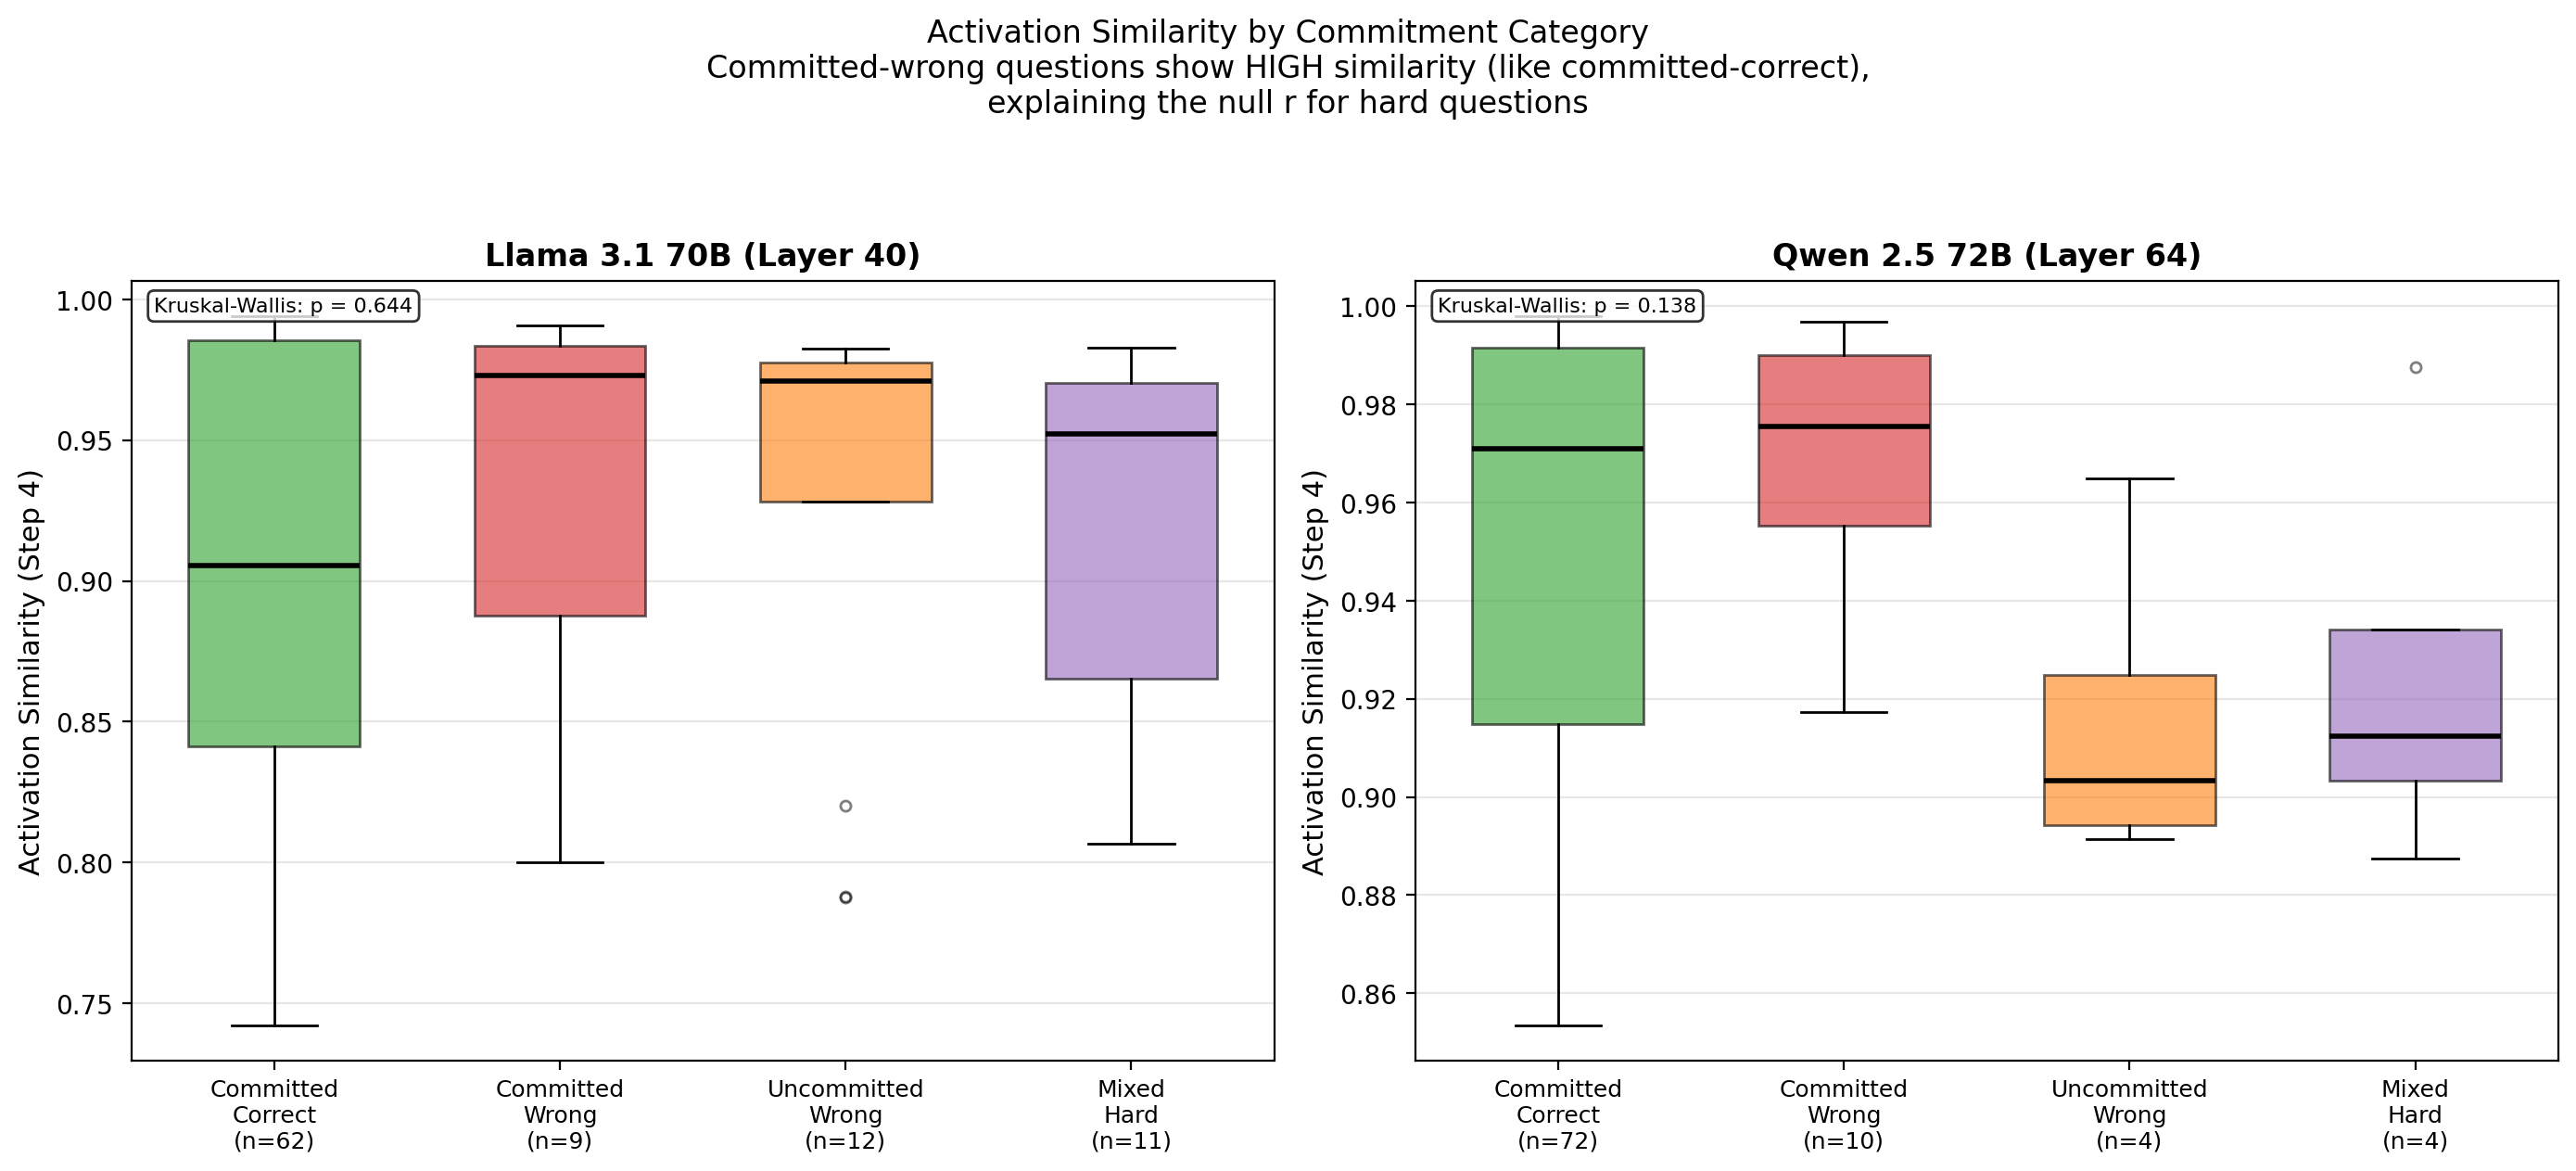
\includegraphics[width=\columnwidth]{figures/commitment_categories_boxplot.png}
\caption{Activation similarity at step~4 by commitment category. Committed-wrong questions (red) show similarity comparable to committed-correct (green), while uncommitted-wrong (orange) trend lower.}
\label{fig:commitment_categories}
\end{figure}

\textbf{Answer agreement.} Activation similarity does not predict answer agreement ($r = -0.13$, $p = 0.22$), confirming the signal reflects \emph{process} consistency (trajectory structure) rather than \emph{output} agreement.

\subsection{Cross-Model Validation}

To test whether representational commitment is architecture-dependent, we run the same experiment on two additional models: Qwen~2.5~72B \citep{qwen2.5}---same depth (80 layers) and hidden dimension (8{,}192) as Llama but a different architecture, tokenizer, and training corpus---and Phi-3-Medium-14B \citep{phi3}---a structurally different model with 40 layers, $d{=}5120$, and 14B parameters. We run all 100 questions with 10 trials each on all three models (988 Llama, 998 Qwen, 1{,}000 Phi-3 trajectories).

The negative correlation replicates in both models. Qwen shows an even stronger peak ($r = -0.65$ at layer~64, 95\% CI $[-0.74, -0.55]$, $p < 10^{-6}$). Phi-3 replicates at step~4 ($r = -0.36$ at layer~16, 95\% CI $[-0.52, -0.17]$, $p = 0.0005$, $n{=}91$), with an even stronger signal at step~5 ($r = -0.58$ at layer~4, 95\% CI $[-0.72, -0.41]$, $p < 10^{-6}$)---the one-step delay plausibly reflecting the smaller model needing additional evidence before committing. Two pieces of evidence support this as a delayed commitment signal rather than a distinct phenomenon: (1)~the step-4-to-step-5 shift mirrors the step-3-to-step-4 shift seen between StrategyQA and HotpotQA for Llama, where the commitment juncture adjusts to the amount of evidence needed; and (2)~the layer profile at Phi-3's step~5 ($r = -0.58$ at layer~4, all layers 4--32 significant) exhibits the same monotonic deepening pattern as Llama's step~4, suggesting the same underlying process operating one step later. All sampled layers 4--36 are significant in Phi-3 at step~4 (all $p < 0.04$; full results in Table~\ref{tab:crossmodel_full}, Appendix~\ref{app:crossmodel}).\footnote{The positive correlation at layer~0 ($r = +0.47$ for Llama, $+0.49$ for Qwen; Table~\ref{tab:crossmodel_full}) reflects input-level similarity rather than representational commitment. At the embedding layer, hidden states are determined almost entirely by the input tokens, which are identical across runs of the same question. Higher embedding-layer similarity therefore indexes questions whose token distributions are more concentrated (typically shorter, simpler questions), which also tend to produce more consistent behavior. This positive correlation is an expected artifact of measuring similarity at the input layer and does not confound the negative correlations at deeper layers, where representations have been transformed by the model's computations. Phi-3 does not show this pattern ($r = -0.05$, $p = .63$), likely due to its different tokenizer and embedding structure.}

\begin{figure}[t]
\centering
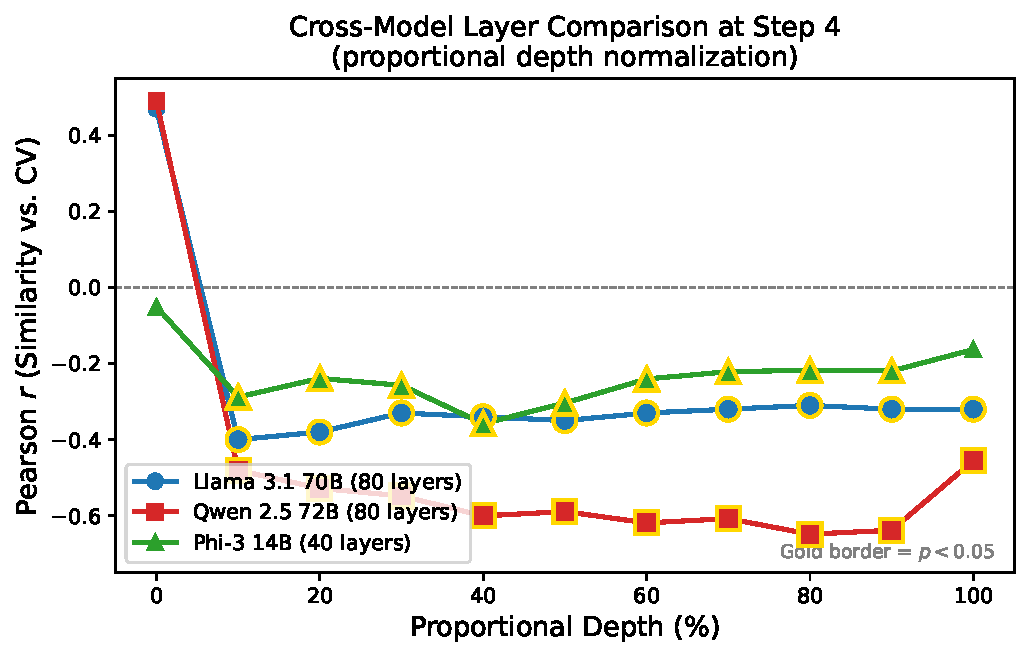
\includegraphics[width=\columnwidth]{figures/cross_model_proportional_depth.pdf}
\caption{Layer-wise correlation between activation similarity and behavioral CV at step~4 for all three models, with layers normalized to proportional depth (layer / max layer $\times$ 100\%) to enable comparison across architectures. All three models show the negative correlation characteristic of representational commitment, with Qwen strongest ($r = -0.65$) and Phi-3 weakest but significant ($r = -0.36$). The positive correlation at 0\% depth (embedding layer) for Llama and Qwen reflects an input-similarity artifact absent in Phi-3 (see text). Gold borders: $p < 0.05$.}
\label{fig:crossmodel}
\end{figure}

Notably, the \emph{peak layer} differs across all three models: Llama peaks at layer~40 (50\% depth), Qwen at layer~64 (80\% depth), and Phi-3 at layer~16 (40\% depth). This suggests representational commitment is a universal phenomenon whose depth profile is architecture-dependent (Figure~\ref{fig:crossmodel}; see also Figure~\ref{fig:step_progression_multimodel} in Appendix~\ref{app:crossmodel} for the temporal profile across all three models). Crucially, Phi-3's validation extends the finding beyond the 70B scale to a 5$\times$ smaller model with half the layer count and a different hidden dimension, ruling out the possibility that the signal is specific to large models or a particular architectural template.

\subsection{Cross-Benchmark Generalization: StrategyQA}

To test whether representational commitment is specific to retrieval-based multi-hop QA, we run the same experiment on StrategyQA \citep{strategyqa}, a benchmark requiring implicit multi-step reasoning with yes/no answers---a different task structure, answer space, and retrieval pattern than HotpotQA. We sample 50 questions (25 yes, 25 no; balanced, $\geq$2 decomposition steps) and run Llama-3.1-70B with 10 runs each (500 trajectories, $T{=}0.5$).

The commitment signal replicates strongly: at step~3, the correlation between activation similarity and behavioral CV reaches $r = -0.83$ (95\% CI $[-0.90, -0.76]$, $p < 10^{-13}$, $n{=}50$), spanning all sampled layers 8--80 (all $|r| > 0.72$, all $p < 10^{-8}$). The signal peaks one step earlier than HotpotQA (step~3 vs.\ step~4), consistent with StrategyQA's shorter reasoning chains (mean 5.1 steps vs.\ ${\sim}12$ for HotpotQA). The partial correlation controlling for accuracy is virtually unchanged ($r = -0.83$, $p < 10^{-13}$), as expected given the high overall accuracy (93.2\%). This rules out the concern that the stronger StrategyQA signal is merely an artifact of higher accuracy: if accuracy were driving the correlation, controlling for it would attenuate the signal, as it does on HotpotQA (raw $r = -0.35 \to$ partial $r = -0.45$). The stability of the partial correlation ($r = -0.83 \to -0.83$) indicates that the stronger signal reflects a genuine difference in how commitment manifests on shorter reasoning chains---the compressed trajectory means the commitment juncture is sharper and less noisy, producing a cleaner signal rather than an accuracy artifact. By step~4, the signal has dissipated ($r \approx 0.07$, $p > 0.7$)---commitment has already occurred. This pattern confirms that the commitment juncture adapts to task structure: it occurs at the step where sufficient evidence has accumulated for the model to form a committed interpretation, regardless of benchmark.

\subsection{Runtime Monitor: Predicting Consistency from Hidden States}

We evaluate whether the commitment signal is strong enough for a practical runtime monitor. We frame consistency prediction as binary classification using LOOCV with logistic regression, testing five hidden-state features and four surface-level baselines under two labeling schemes: \emph{quintile} (top/bottom 20\% by CV) and \emph{median split} (full results in Table~\ref{tab:runtime_full}, Appendix~\ref{app:runtime}).

Hidden-state features achieve strong discrimination across both models. Under quintile labeling, a per-layer similarity profile reaches AUROC = 0.97 [0.90, 1.00] on Llama, and PCA-reduced hidden states reach 0.93 [0.85, 0.99] on Qwen. Under median split, PCA features achieve 0.85 on Llama and layer-averaged similarity reaches 0.88 on Qwen. All surface-level baselines (question length, context size, thought length) remain near or below chance (AUROC $\leq 0.65$), confirming that the discriminative signal resides in hidden states, not surface properties. Qwen's scalar similarity features perform well even under median split (AUROC $\approx$ 0.86--0.88), consistent with its stronger raw correlation. Figure~\ref{fig:runtime_roc} shows ROC curves.

\begin{figure}[t]
\centering
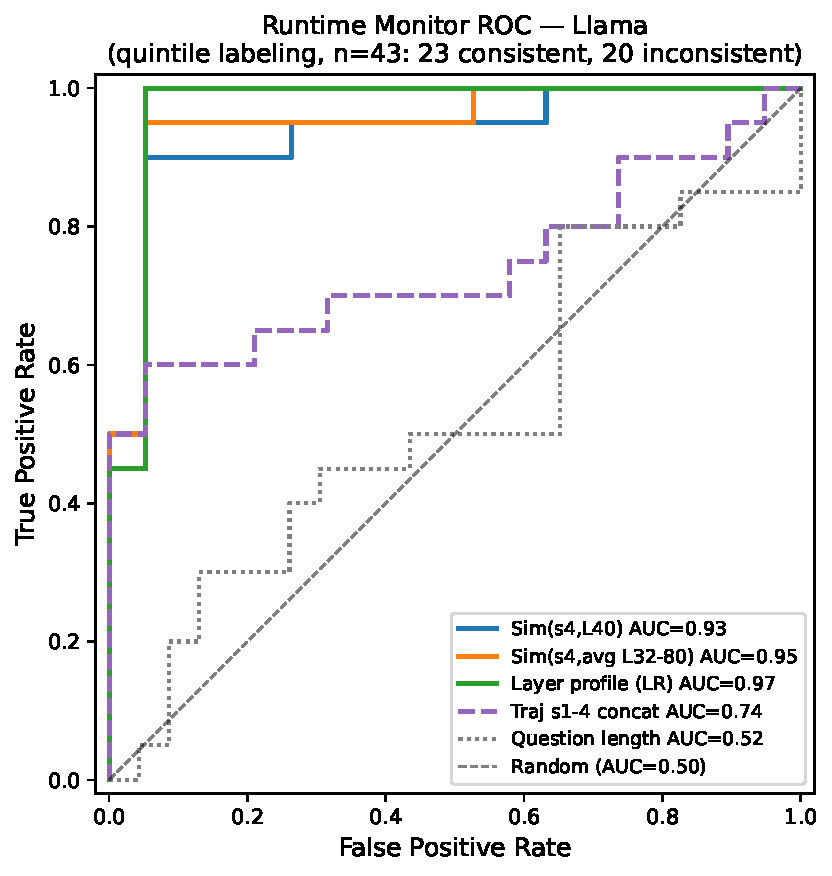
\includegraphics[width=0.48\columnwidth]{figures/runtime_monitor_roc_llama_quintile.pdf}
\hfill
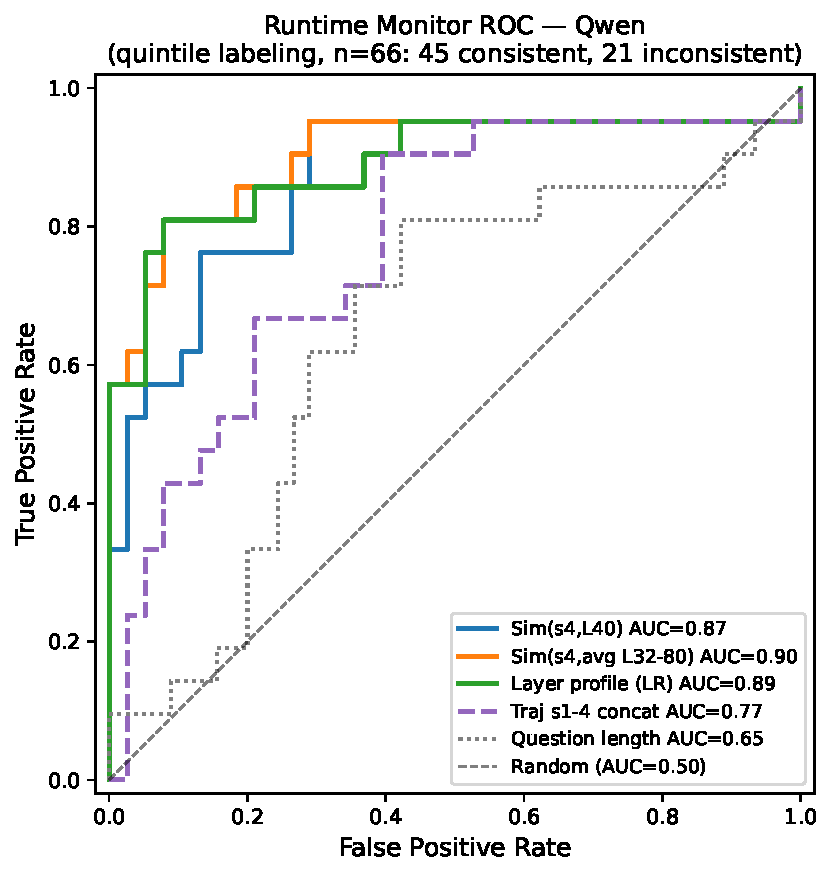
\includegraphics[width=0.48\columnwidth]{figures/runtime_monitor_roc_qwen_quintile.pdf}
\caption{ROC curves for runtime consistency prediction (quintile labeling). Hidden-state features (solid) substantially outperform surface baselines (dashed).}
\label{fig:runtime_roc}
\end{figure}

A runtime monitor using only step-4 hidden states---available before the trajectory completes---can flag questions likely to produce inconsistent behavior, enabling selective retry or human oversight.

\subsection{Intervention: Inducing Representational Commitment}
\label{sec:intervention}

If representational commitment causally drives behavioral consistency, then inducing commitment should reduce downstream variance. We test this with a prompting intervention: at step~3 of the ReAct trajectory---one step before the commitment juncture---we append an instruction to the agent's observation requiring it to explicitly commit to a reasoning strategy before proceeding.\footnote{The full prompt reads: ``Based on the evidence you have gathered so far, commit to a specific reasoning strategy for solving this question. State your committed strategy clearly in your next Thought, then follow through with it. Do not change strategies or start over---build on what you have learned.''} The control condition uses the standard ReAct agent with no modification.

We run both conditions on 100 HotpotQA questions (the same set used in the Qwen cross-model validation) with 10 runs per question per condition on Llama~3.1~70B ($T = 0.5$), extracting hidden states identically to the main experiment. Table~\ref{tab:intervention} reports the results.

\begin{table}[h]
\centering
\caption{Prompting intervention results ($n = 100$ questions, 10 runs each). The commitment prompt significantly reduces behavioral CV without affecting accuracy. Effect is strongest for originally-inconsistent questions.}
\label{tab:intervention}
\small
\begin{tabular}{lcccccc}
\toprule
\textbf{Metric} & \textbf{Control} & \textbf{Commitment} & \textbf{$\Delta$} & \textbf{$d$} & \textbf{$p$} \\
\midrule
Behavioral CV & 0.112 & 0.094 & $-$0.018 & 0.21 & .037 \\
Action seq.\ diversity & 0.250 & 0.223 & $-$0.027 & 0.23 & .026 \\
Accuracy & 0.835 & 0.823 & $-$0.012 & 0.14 & .164 \\
\bottomrule
\end{tabular}
\end{table}

The commitment prompt reduces step-count CV by 16\% (paired $t(99) = 2.12$, $p = .037$, Cohen's $d = 0.21$; Wilcoxon $p = .033$) and action sequence diversity by 11\% ($d = 0.23$, $p = .026$), with no significant accuracy change ($p = .164$). The intervention makes behavior more consistent without degrading task performance.

\textbf{Stratified analysis.} The effect concentrates where it matters most. Splitting questions into tertiles by control-condition CV: originally-inconsistent questions (top tertile, $n = 32$) show the largest CV reduction ($0.270 \to 0.189$, $\Delta = 0.080$, $p < .001$), while originally-consistent questions (bottom tertile, $n = 40$, CV $= 0.000$) show a small floor-effect increase ($0.000 \to 0.026$, $p = .007$). The middle tertile shows no significant change. This pattern---large effects on inconsistent questions, negligible effects on already-consistent ones---is precisely what a commitment mechanism predicts: the intervention induces commitment where the model was previously uncommitted, but has little to add where commitment already exists.

\subsection{Preliminary Steering Experiment}

If representational commitment has a directional signature in activation space, it should be possible to steer the model toward more committed states directly. We conduct a preliminary experiment: for 5 questions, we extract the ``commitment direction'' as the difference between mean hidden states of committed (consistent-correct) and uncommitted (inconsistent) runs at step~4, layer~40. We then add this direction (scaled by $\alpha = 1.5$) to hidden states during inference.

Results are mixed: on 2/5 questions, steering reduced step-count CV (from 0.31 to 0.18 and 0.27 to 0.12), while on 3/5 questions, steering either had no effect or slightly increased variance. The intervention occasionally disrupted coherent reasoning, producing malformed tool calls. We interpret this as reflecting a fundamental asymmetry between prompting and activation interventions in the multi-step setting. The prompting intervention succeeds because it changes what the model \emph{generates} at step~3: the explicit commitment text becomes part of the context window, shaping how hidden states evolve across \emph{all} layers in subsequent forward passes. Steering at a single layer at step~4 intervenes too late and too locally---it statically shifts representations at one point in the network after the commitment juncture has already passed, rather than changing the information flow through the full forward pass during the critical step. This suggests that representational commitment is not a localized activation pattern amenable to single-site perturbation, but a distributed computational process that unfolds across layers and steps. Multi-layer, multi-step steering \citep{zou2023repe} or representation finetuning may be required to achieve activation-level consistency improvements.

%%%%%%%%%%%%%%%%%%%%%%%%%%%%%%%%%%%%%%%%%%%%%%%%%%%%%%%%%%%%%%%%%%%%%%%%%%%%%%%
\section{Discussion}
%%%%%%%%%%%%%%%%%%%%%%%%%%%%%%%%%%%%%%%%%%%%%%%%%%%%%%%%%%%%%%%%%%%%%%%%%%%%%%%

\textbf{Representational commitment as a new axis.} Recent work has identified linear directions in activation space encoding behavioral properties: persona vectors for character traits \citep{anthropic_persona}, the assistant axis for default model behavior \citep{anthropic_axis}, and truth directions for factual accuracy \citep{marks2024geometry}. Our finding suggests \emph{commitment}---the degree to which a model integrates observations---may constitute another such axis relevant to agent reliability. Unlike persona or truth, which are static properties of model weights, commitment is a dynamic property that emerges and resolves during multi-step interaction, making it specifically relevant to agentic rather than single-turn settings. The prompting intervention (Section~\ref{sec:intervention}) provides experimental evidence that this property is not merely correlational: inducing commitment at step~3 causally reduces downstream behavioral variance.

\textbf{Why step~4?} Steps 1--3 involve initial queries that return limited information. By step~4, the model has received 3--4 observations and must integrate them into a coherent interpretation. This is the commitment juncture: models that update their representations proceed consistently; those that do not, diverge. The signal fading at step~5 suggests that by then, trajectories have already committed or scattered beyond the point where hidden states carry a clean signal.

\textbf{Single-turn vs.\ multi-step probing.} A key negative finding: correctness probes that work in single-turn settings \citep{gnosis, stickland2024reasoning} fail in our multi-step agentic setting. We confirmed this with a direct comparison: single-turn probing on the same questions achieves AUC = 0.35, even worse than multi-step. The failure is not caused by context accumulation but by correctness being question-determined. This highlights a gap in the probing literature that assumes within-input variance exists.

\textbf{Cross-model and cross-benchmark universality.} Replication on Qwen~2.5~72B and Phi-3-Medium-14B---models spanning different architectures, scales (14B--72B), layer counts (40--80), and hidden dimensions (5120--8192)---confirms that representational commitment is not specific to any single model family or scale. The different peak layers (Llama: layer~40, 50\% depth; Qwen: layer~64, 80\% depth; Phi-3: layer~16, 40\% depth) suggest that \emph{where} commitment manifests is architecture-dependent, but \emph{that} it manifests is universal. Phi-3's one-step-later peak ($r = -0.58$ at step~5 vs.\ step~4 for the 70B models) may reflect smaller models requiring additional evidence accumulation before committing; we note that this interpretation is consistent with, but not proven by, the current data---a definitive test would require varying the amount of evidence available at each step while controlling for model scale. Qwen's uniformly stronger signal ($r = -0.65$ vs.\ $-0.35$ at peak) may reflect its higher accuracy (81\% vs.\ 70\%), producing more questions in the ``committed correct'' regime where the signal is strongest. Cross-benchmark validation on StrategyQA---a task with different structure (implicit reasoning, yes/no answers) and shorter chains---produces the strongest signal of any condition ($r = -0.83$) with the commitment juncture shifting to step~3, demonstrating that the phenomenon adapts to task structure rather than being anchored to a fixed step.

\textbf{Limitations.} Our study validates on three models (14B--72B) across two benchmarks (HotpotQA and StrategyQA); broader task coverage (e.g., code generation, mathematical reasoning) would further strengthen the claims. CV of step counts is a coarse consistency proxy; sequence-level metrics may reveal finer structure. The prompting intervention is confounded by additional tokens in the context window; activation-level steering would provide cleaner causal evidence but remains technically challenging (Section~4.8). While the partial correlation analysis rules out task difficulty, unmeasured confounders may exist. All models are instruction-tuned; base model behavior is unknown.

\textbf{Future directions.} Three directions follow: (1)~circuit tracing at divergence points using attribution graphs \citep{anthropic_circuits} to identify the computations underlying representational commitment; (2)~multi-layer activation steering to achieve consistency improvements without prompt modifications; and (3)~consistency-aware training via DPO on committed vs.\ uncommitted trajectories.

%%%%%%%%%%%%%%%%%%%%%%%%%%%%%%%%%%%%%%%%%%%%%%%%%%%%%%%%%%%%%%%%%%%%%%%%%%%%%%%
\section{Conclusion}
%%%%%%%%%%%%%%%%%%%%%%%%%%%%%%%%%%%%%%%%%%%%%%%%%%%%%%%%%%%%%%%%%%%%%%%%%%%%%%%

Behavioral consistency in LLM agents has a measurable internal signature. At step~4 of a ReAct trajectory, the degree to which hidden states differentiate across runs---what we call \emph{representational commitment}---predicts downstream behavioral consistency. This signal survives difficulty controls (partial $r = -0.45$, 95\% CI $[-0.59, -0.29]$), is robust to permutation testing ($p < 0.001$), and produces a 4.1$\times$ effect between extreme quartiles ($d = 1.01$). It is not explained by simple baselines. It predicts consistency but not correctness, establishing it as a relational property of agent representations. Cross-model validation on Qwen~2.5~72B ($r = -0.65$) and Phi-3-Medium-14B ($r = -0.36$)---spanning 14B to 72B parameters, 40 to 80 layers, and three distinct architectures---confirms the signal generalizes across model families and scales. Cross-benchmark validation on StrategyQA ($r = -0.83$, $n{=}50$) extends this to a different task type, with the commitment juncture shifting to step~3 consistent with shorter reasoning chains. A runtime monitor built on these features achieves AUROC up to 0.97, and a prompting intervention inducing commitment reduces behavioral variance by 16\% overall (30\% on originally-inconsistent questions) without affecting accuracy. These findings bridge behavioral agent evaluation and mechanistic interpretability, demonstrating that representational commitment is not only a measurable phenomenon but a practically exploitable signal for monitoring and improving agent reliability.

%%%%%%%%%%%%%%%%%%%%%%%%%%%%%%%%%%%%%%%%%%%%%%%%%%%%%%%%%%%%%%%%%%%%%%%%%%%%%%%

\paragraph{Author Note.} Large language models (specifically Claude) were used for code generation, data analysis scripting, and writing assistance during the preparation of this manuscript. All scientific claims, experimental designs, and interpretations were made by the authors.

\bibliography{references}
\bibliographystyle{colm2026_conference}

\appendix

\section{Permutation Test Results}
\label{app:permutation}

\begin{table}[h]
\caption{Permutation test at step~4 (10{,}000 iterations). All layers 32--80 are significant at $p < 0.002$.}
\label{tab:permutation}
\centering
\small
\begin{tabular}{lccc}
\toprule
Layer & $r$ & Param.\ $p$ & Perm.\ $p$ \\
\midrule
32 & $-0.340$ & $0.0008$ & $0.0007$ \\
\textbf{40} & $\mathbf{-0.348}$ & $\mathbf{0.0006}$ & $\mathbf{0.0003}$ \\
48 & $-0.326$ & $0.0013$ & $0.0012$ \\
56 & $-0.320$ & $0.0017$ & $0.0011$ \\
64 & $-0.313$ & $0.0021$ & $0.0014$ \\
72 & $-0.316$ & $0.0019$ & $0.0019$ \\
80 & $-0.319$ & $0.0017$ & $0.0019$ \\
\bottomrule
\end{tabular}
\end{table}

\section{Partial Correlation Results}
\label{app:partial}

\begin{table}[h]
\caption{Partial correlations at step~4, controlling for accuracy and difficulty label. The signal strengthens after removing difficulty-related variance.}
\label{tab:partial}
\centering
\small
\begin{tabular}{lcccc}
\toprule
Layer & Raw $r$ & Raw $p$ & Partial $r$ & Partial $p$ \\
\midrule
32 & $-0.340$ & $.0008$ & $-0.456$ & $< .0001$ \\
\textbf{40} & $\mathbf{-0.348}$ & $\mathbf{.0006}$ & $\mathbf{-0.445}$ & $\mathbf{< .0001}$ \\
48 & $-0.326$ & $.0013$ & $-0.416$ & $< .0001$ \\
56 & $-0.320$ & $.0017$ & $-0.399$ & $< .0001$ \\
64 & $-0.313$ & $.0021$ & $-0.387$ & $.0001$ \\
72 & $-0.316$ & $.0019$ & $-0.387$ & $.0001$ \\
80 & $-0.319$ & $.0017$ & $-0.375$ & $.0002$ \\
\bottomrule
\end{tabular}
\end{table}

\section{Full Cross-Model Layer-Wise Results}
\label{app:crossmodel}

Table~\ref{tab:crossmodel_full} reports the full layer-wise correlations between activation similarity and behavioral CV at step~4 for all three models. Phi-3 layers are mapped to proportionally equivalent depths (e.g., Phi-3 layer~16 $\approx$ 40\% depth).

\begin{table}[h]
\caption{Cross-model validation at step~4. All three models show the negative correlation between activation similarity and behavioral CV. Phi-3 (14B, 40 layers, $d{=}5120$) validates on a structurally different architecture. $^*p < 0.05$.}
\label{tab:crossmodel_full}
\centering
\small
\begin{tabular}{lcccccc}
\toprule
 & \multicolumn{2}{c}{Llama 3.1 70B} & \multicolumn{2}{c}{Qwen 2.5 72B} & \multicolumn{2}{c}{Phi-3 14B} \\
\cmidrule(lr){2-3} \cmidrule(lr){4-5} \cmidrule(lr){6-7}
Layer & $r$ & $p$ & $r$ & $p$ & $r$ & $p$ \\
\midrule
0  & $0.47^*$ & $< .001$ & $0.49^*$ & $< .001$ & $-0.05$ & $.634$ \\
8  & $-0.40^*$ & $< .001$ & $-0.48^*$ & $< .001$ & $-0.24^*$ & $.023$ \\
16 & $-0.38^*$ & $< .001$ & $-0.53^*$ & $< .001$ & $\mathbf{-0.36^*}$ & $\mathbf{< .001}$ \\
24 & $-0.33^*$ & $.001$ & $-0.55^*$ & $< .001$ & $-0.24^*$ & $.022$ \\
32 & $-0.34^*$ & $< .001$ & $-0.60^*$ & $< .001$ & $-0.22^*$ & $.038$ \\
\textbf{40} & $\mathbf{-0.35^*}$ & $\mathbf{< .001}$ & $-0.59^*$ & $< .001$ & $-0.16$ & $.123$ \\
48 & $-0.33^*$ & $.001$ & $-0.62^*$ & $< .001$ & --- & --- \\
56 & $-0.32^*$ & $.002$ & $-0.61^*$ & $< .001$ & --- & --- \\
\textbf{64} & $-0.31^*$ & $.002$ & $\mathbf{-0.65^*}$ & $\mathbf{< .001}$ & --- & --- \\
72 & $-0.32^*$ & $.002$ & $-0.64^*$ & $< .001$ & --- & --- \\
80 & $-0.32^*$ & $.002$ & $-0.46^*$ & $< .001$ & --- & --- \\
\midrule
Sig.\ layers & \multicolumn{2}{c}{11 / 11} & \multicolumn{2}{c}{11 / 11} & \multicolumn{2}{c}{4 / 6} \\
Peak $r$ & \multicolumn{2}{c}{$-0.35$ (L40)} & \multicolumn{2}{c}{$-0.65$ (L64)} & \multicolumn{2}{c}{$-0.36$ (L16)} \\
Accuracy & \multicolumn{2}{c}{0.70} & \multicolumn{2}{c}{0.81} & \multicolumn{2}{c}{0.69} \\
\bottomrule
\end{tabular}
\end{table}

Figure~\ref{fig:step_progression_multimodel} shows the temporal profile of the commitment signal across all three models. Each model is plotted at its peak layer. The 70B models (Llama and Qwen) reach their strongest signal at step~4, while Phi-3 (14B) peaks one step later at step~5, consistent with the smaller model requiring additional evidence before committing.

\begin{figure}[h]
\centering
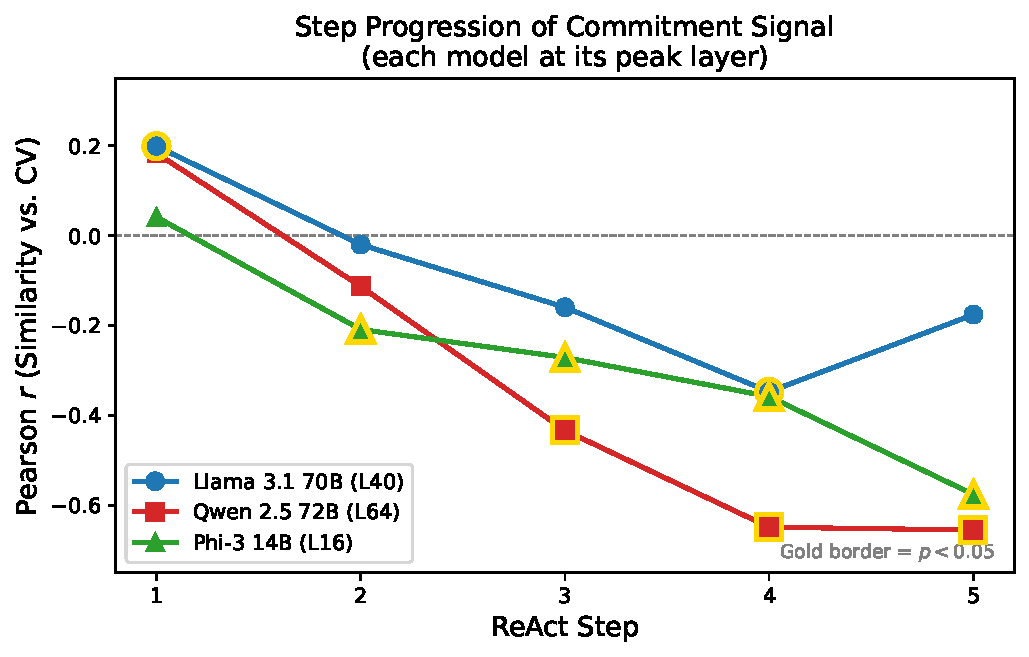
\includegraphics[width=0.8\columnwidth]{figures/multi_model_step_progression.pdf}
\caption{Step progression of the commitment signal across three models (each at its peak layer: Llama L40, Qwen L64, Phi-3 L16). Both 70B models peak at step~4 while Phi-3 (14B) peaks at step~5, suggesting smaller models require one additional evidence-gathering step before committing. Gold borders: $p < 0.05$.}
\label{fig:step_progression_multimodel}
\end{figure}

\section{Commitment Category Visualization}
\label{app:tsne}

Figure~\ref{fig:tsne} shows a t-SNE visualization of step-4 hidden states (layer~40) for all 100 questions, colored by commitment category. Left panel: Llama~3.1~70B; right panel: Qwen~2.5~72B. Hidden states are first reduced to 50 dimensions via PCA, then projected to 2D via t-SNE (perplexity~30). Each point represents one question's mean hidden state across its 10 runs. Committed-correct (green) and committed-wrong (red) questions occupy overlapping regions of the representation space, consistent with our finding that commitment is correctness-agnostic (Section~4.4). Uncommitted-wrong questions (orange) tend toward more diffuse regions, reflecting their higher activation variance.

\begin{figure}[h]
\centering
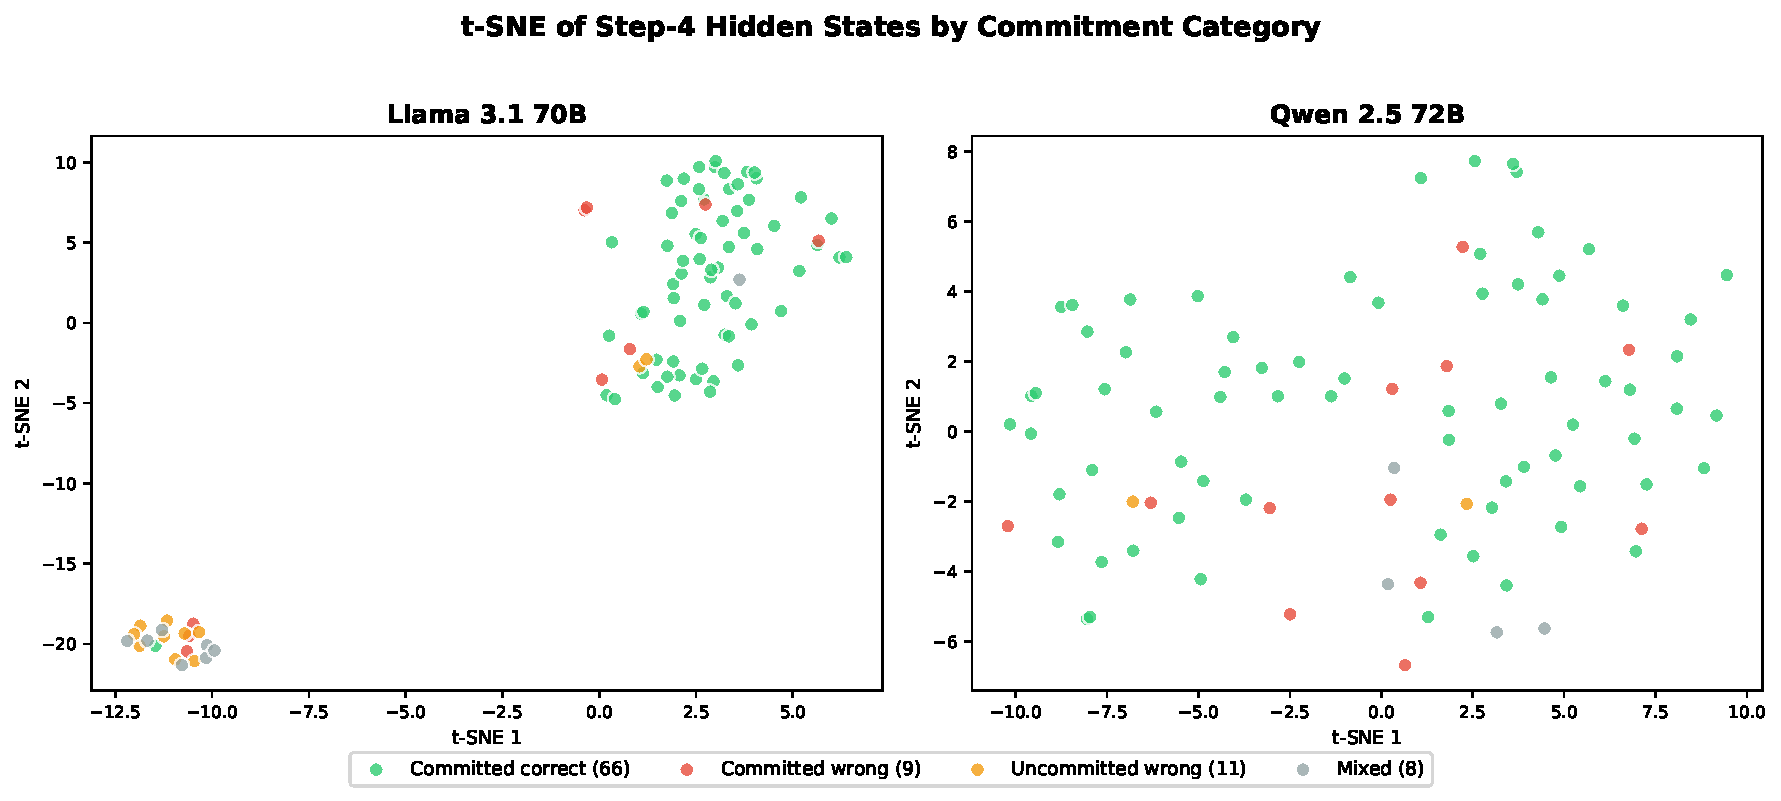
\includegraphics[width=\columnwidth]{figures/commitment_tsne.pdf}
\caption{t-SNE projection of step-4 hidden states (PCA to 50D, then t-SNE to 2D) colored by commitment category. Committed-correct (green) and committed-wrong (red) overlap, confirming that representational commitment is orthogonal to correctness. Uncommitted-wrong (orange) questions show more dispersed representations.}
\label{fig:tsne}
\end{figure}

\section{Baseline Predictors of Behavioral CV}
\label{app:baselines}

Table~\ref{tab:baselines_full} reports the full set of candidate predictors of behavioral CV, including input-level features and downstream behavioral consequences.

\begin{table}[h]
\caption{Predictors of behavioral CV. $\dagger$Downstream behavioral consequences, not confounds.}
\label{tab:baselines_full}
\centering
\small
\begin{tabular}{lrr}
\toprule
Predictor & $r$ & $p$ \\
\midrule
\textbf{Hidden-state sim.\ (S4, L40)} & $\mathbf{-0.35}$ & $\mathbf{.0006}$ \\
\midrule
Accuracy (correct rate)$^\dagger$ & $-0.31$ & $.002$ \\
Mean total thought length$^\dagger$ & $0.26$ & $.011$ \\
Mean search actions$^\dagger$ & $0.23$ & $.019$ \\
Mean step count$^\dagger$ & $0.21$ & $.037$ \\
\midrule
Question word count & $0.10$ & $.31$ \\
Question char count & $0.12$ & $.25$ \\
N context documents & $0.04$ & $.66$ \\
Mean thought length (S3) & $0.12$ & $.24$ \\
\bottomrule
\end{tabular}
\end{table}

\section{Runtime Monitor: Full Results}
\label{app:runtime}

Table~\ref{tab:runtime_full} reports the complete runtime monitor evaluation across all features, models, and labeling schemes.

\begin{table}[h]
\caption{Runtime monitor AUROC (95\% CI) for predicting behavioral consistency. Features A--E use step-4 hidden states; baselines use only surface-level input properties.}
\label{tab:runtime_full}
\centering
\small
\begin{tabular}{lcccc}
\toprule
 & \multicolumn{2}{c}{Llama 3.1 70B} & \multicolumn{2}{c}{Qwen 2.5 72B} \\
\cmidrule(lr){2-3} \cmidrule(lr){4-5}
Feature & Quintile & Median & Quintile & Median \\
\midrule
A: Sim (L40) & .93 & .55 & .87 & .86 \\
B: Sim (avg) & .95 & .58 & .90 & .88 \\
C: Layer profile & \textbf{.97} & .73 & .89 & .88 \\
D: Trajectory & .74 & .55 & .77 & .79 \\
E: PCA (L40) & .94 & \textbf{.85} & \textbf{.93} & .67 \\
\midrule
Random & .43 & .57 & .48 & .48 \\
Question length & .52 & .60 & .65 & .57 \\
Context docs & .08 & .06 & .07 & .06 \\
Thought length & .10 & .04 & .00 & .00 \\
\bottomrule
\end{tabular}
\end{table}

\section{StrategyQA Cross-Benchmark Results}
\label{app:strategyqa}

Table~\ref{tab:strategyqa_layers} reports the full layer-wise correlations between activation similarity and behavioral CV at step~3 (the peak step) for Llama-3.1-70B on StrategyQA ($n{=}50$). All layers 8--80 are significant at $p < 10^{-8}$, with partial correlations controlling for accuracy virtually unchanged due to the high overall accuracy (93.2\%).

\begin{table}[h]
\caption{StrategyQA: Layer-wise correlations at step~3 (Llama-3.1-70B, $n{=}50$). The signal spans all non-embedding layers and peaks at layer~72. Partial correlations control for accuracy.}
\label{tab:strategyqa_layers}
\centering
\small
\begin{tabular}{lcccc}
\toprule
Layer & Raw $r$ & Raw $p$ & Partial $r$ & Partial $p$ \\
\midrule
0  & --- & --- & --- & --- \\
8  & $-0.73$ & $2.5 \times 10^{-9}$ & $-0.72$ & $2.9 \times 10^{-9}$ \\
16 & $-0.78$ & $3.8 \times 10^{-11}$ & $-0.77$ & $4.3 \times 10^{-11}$ \\
24 & $-0.76$ & $2.3 \times 10^{-10}$ & $-0.75$ & $3.7 \times 10^{-10}$ \\
32 & $-0.78$ & $2.6 \times 10^{-11}$ & $-0.78$ & $4.0 \times 10^{-11}$ \\
40 & $-0.81$ & $8.7 \times 10^{-13}$ & $-0.81$ & $8.4 \times 10^{-13}$ \\
48 & $-0.82$ & $2.0 \times 10^{-13}$ & $-0.82$ & $1.9 \times 10^{-13}$ \\
56 & $-0.83$ & $8.8 \times 10^{-14}$ & $-0.83$ & $9.7 \times 10^{-14}$ \\
64 & $-0.83$ & $7.7 \times 10^{-14}$ & $-0.83$ & $9.3 \times 10^{-14}$ \\
\textbf{72} & $\mathbf{-0.83}$ & $\mathbf{7.4 \times 10^{-14}}$ & $\mathbf{-0.83}$ & $\mathbf{9.1 \times 10^{-14}}$ \\
80 & $-0.82$ & $4.8 \times 10^{-13}$ & $-0.82$ & $4.7 \times 10^{-13}$ \\
\bottomrule
\end{tabular}
\end{table}

Table~\ref{tab:crossbenchmark} summarizes cross-benchmark comparison. The StrategyQA signal is stronger than HotpotQA despite a smaller sample, and peaks one step earlier consistent with its shorter reasoning chains.

\begin{table}[h]
\caption{Cross-benchmark comparison of the representational commitment signal (Llama-3.1-70B). StrategyQA produces a stronger signal that peaks one step earlier, consistent with shorter reasoning chains.}
\label{tab:crossbenchmark}
\centering
\small
\begin{tabular}{lcc}
\toprule
 & HotpotQA & StrategyQA \\
\midrule
Task type & Multi-hop retrieval QA & Implicit reasoning \\
Answer type & Span extraction & Yes/no \\
$n$ (questions) & 100 & 50 \\
Runs per question & 10 & 10 \\
Mean chain length & ${\sim}12$ steps & 5.1 steps \\
Accuracy & 70\% & 93.2\% \\
\midrule
Peak step & 4 & 3 \\
Peak layer & 40 & 72 \\
Peak $r$ & $-0.35$ & $-0.83$ \\
95\% CI & $[-0.48, -0.17]$ & $[-0.90, -0.76]$ \\
Peak $p$ & $< 0.001$ & $< 10^{-13}$ \\
Partial $r$ & $-0.45$ & $-0.83$ \\
Sig.\ layers & 7 / 11 & 10 / 11 \\
\bottomrule
\end{tabular}
\end{table}

Figure~\ref{fig:strategyqa_heatmap} shows the step$\times$layer heatmap of Pearson correlations between activation similarity and behavioral CV for StrategyQA, revealing the sharp commitment signal concentrated at step~3 across all layers.

\begin{figure}[h]
\centering
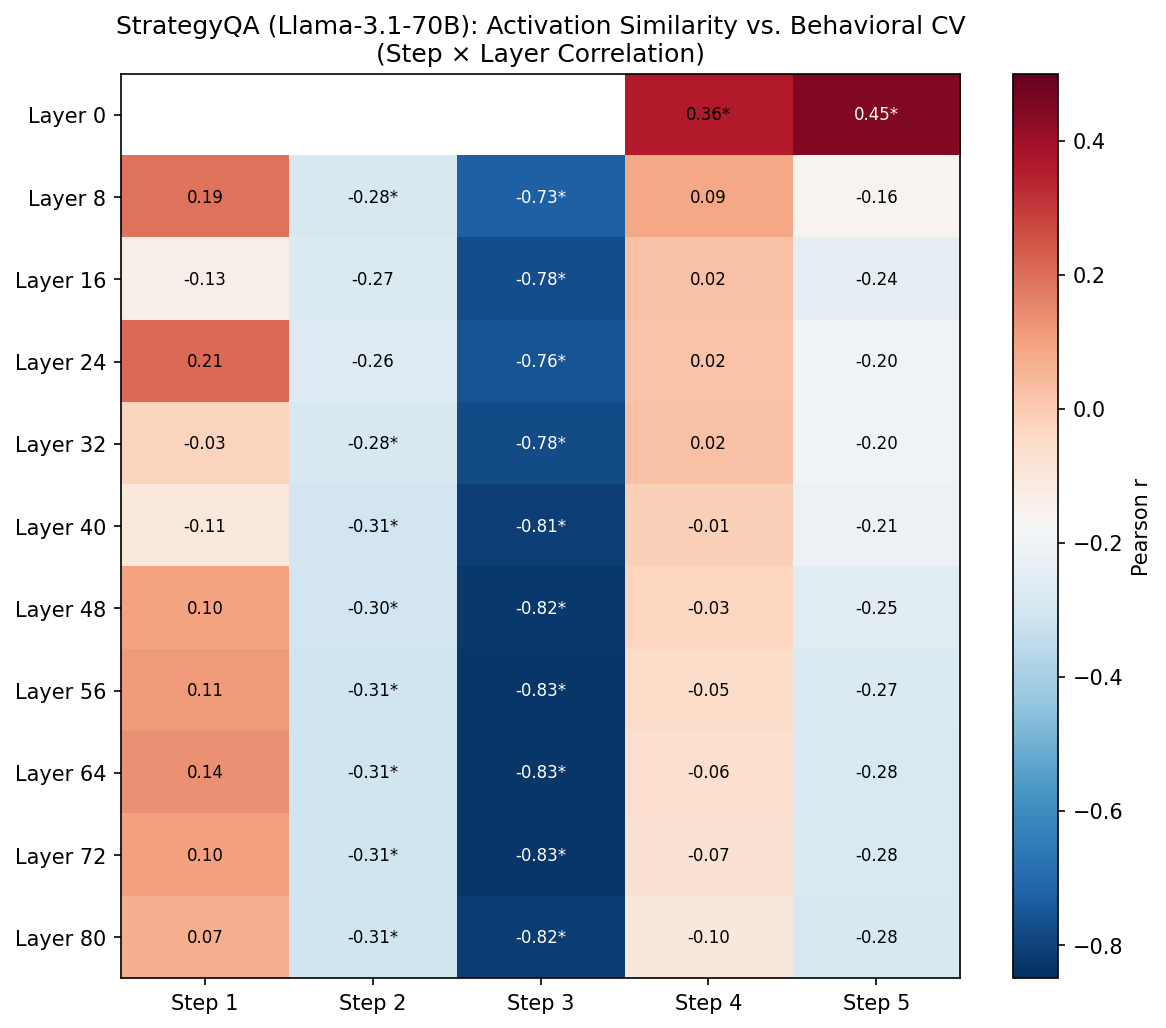
\includegraphics[width=0.7\columnwidth]{figures/strategyqa_heatmap.png}
\caption{StrategyQA step$\times$layer correlation heatmap (Llama-3.1-70B, $n{=}50$). The commitment signal concentrates at step~3 (deep blue column), one step earlier than HotpotQA's step~4 peak, consistent with shorter reasoning chains. All layers 8--80 at step~3 show $|r| > 0.72$ ($p < 10^{-8}$). $^*p < 0.05$.}
\label{fig:strategyqa_heatmap}
\end{figure}

\end{document}
